
%***************************************************************************
%
% CreditCruncher - A portfolio credit risk valorator
% Copyright (C) 2007 Gerard Torrent
%
% This program is free software; you can redistribute it and/or
% modify it under the terms of the GNU General Public License
% as published by the Free Software Foundation; either version 2
% of the License.
%
% This program is distributed in the hope that it will be useful,
% but WITHOUT ANY WARRANTY; without even the implied warranty of
% MERCHANTABILITY or FITNESS FOR A PARTICULAR PURPOSE.  See the
% GNU General Public License for more details.
%
% You should have received a copy of the GNU General Public License
% along with this program; if not, write to the Free Software
% Foundation, Inc., 59 Temple Place - Suite 330, Boston, MA 02111-1307, USA.
%
%
% ccruncher.tex - TeX documentation file - $Rev$
% --------------------------------------------------------------------------
%
% 2007/07/25 - Gerard Torrent [gerard@mail.generacio.com]
%   . initial release
%
%***************************************************************************

\documentclass[a4paper,12pt,final]{article}
\usepackage{times}
\usepackage{latexsym}
\usepackage{amssymb}
\usepackage{abstract}
\usepackage[dvips]{graphicx}
\usepackage[american]{babel}
\usepackage[final]{listings}
\usepackage{fancyhdr}
\usepackage[flushmargin]{footmisc}

%-----------------------------------------------------
% defining some useful values
%-----------------------------------------------------
\def\numversion{1.1}
\def\svnversion{R381}

%-----------------------------------------------------
% some format directives
%-----------------------------------------------------
\sloppy
\pagestyle{fancy}
\setlength\parindent{0ex}

%-----------------------------------------------------
% finally, the doc begins here
%-----------------------------------------------------
\begin{document}


\title{CreditCruncher - Technical Document}
\author{Gerard Torrent Gironella\\\\Version \numversion\ -\ \svnversion}
\date{}
\maketitle


%===========================================================================
\begin{abstract}
The CCruncher goal is compute the credit risk of portfolios where 
investments are fixed income assets taking into account default correlations
between sectors. This is done determining the probability distribution of the 
portfolio loss at time $T$ using Monte Carlo simulation method and computing 
risk statistics over there (Expected Loss, Standard Deviation, Value at Risk,
Expected Shortfall).
\newline
\newline
\textbf{Keywords}: credit risk, Monte Carlo, gaussian copula, Value at Risk,
Expected Shortfall.
\end{abstract}


%===========================================================================
\section{Parameters}

%---------------------------------------------------------------------------
\subsection{Time}
In order to speed up the calculations we precomputes asset losses at fixed 
times. To fix this time nodes we need an \emph{initial date}, the 
\emph{number of steps} and the \emph{step length}. The probability distribution
is computed at date $T = initial\ date + number\ of\ steps \times step\ length$.

\begin{figure}[!hb]
\begin{center}
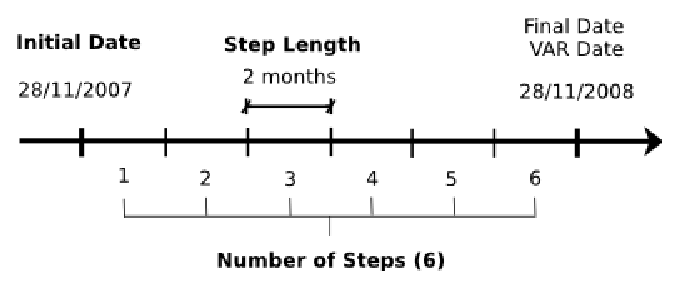
\includegraphics[height=3.0cm, angle=0]{./images/cctime1.eps}
%\caption{Time nodes}
\label{cctime1}
\end{center}
\end{figure}

%---------------------------------------------------------------------------
\subsection{Ratings and Survival Functions}
A credit rating tells a lender or investor the probability of the subject being 
able to pay back a loan. A poor credit rating indicates a high risk of defaulting.
Every rating has associated a survival function. This function indicates the 
probability that a borrower with initial rating $X$ be non-defaulted at time $t$.
The rating system creation and the construction of the survivals functions is 
outside the scope of this paper\footnote{Appendix \ref{ap:tmatrix} shows 
how determine the survival functions using the transition matrix.}.

\begin{figure}[!hb]
\begin{center}
\includegraphics[height=10cm, angle=-90]{./images/survival.ps}
\caption{Survival functions}
\label{survival}
\end{center}
\end{figure}

%---------------------------------------------------------------------------
\subsection{Sectors and correlations}
The risk of a credit portfolio depends crucially on defaults correlations between 
economic sectors. Sectors are groupings of companies that react similarly to 
given economic conditions. Sectors examples are: energy, financial, technology, 
media and entertainment, utilities, health care, etc. Default correlation between 
sectors measures the dependence to default between the defined sectors. This can 
be expressed in table form where 
$\rho_{i,j} = Corr(Sector_i, Sector_j)$:

\begin{center}
\begin{tabular}[]{c|ccc}
             & $Sector_1$     & $\dots$  & $Sector_{m}$   \cr
\hline
$Sector_1$   & $\rho_{1,1}$ & $\dots$  & $\rho_{1,m}$ \cr
$\vdots$     & $\vdots$     & $\ddots$ & $\vdots$     \cr
$Sector_{m}$ & $\rho_{1,m}$ & $\dots$  & $\rho_{m,m}$ \cr
\end{tabular}
\end{center}

%---------------------------------------------------------------------------
\subsection{Portfolio}
Portfolio is composed by borrowers where each one has an initial rating and 
belongs to a sector. Each borrower have one or more assets. Each asset
is defined by the date when it was incorporated in the portfolio, a expected
cashflow and a forecasted recovery at certain dates.

\begin{figure}[!hb]
\begin{center}
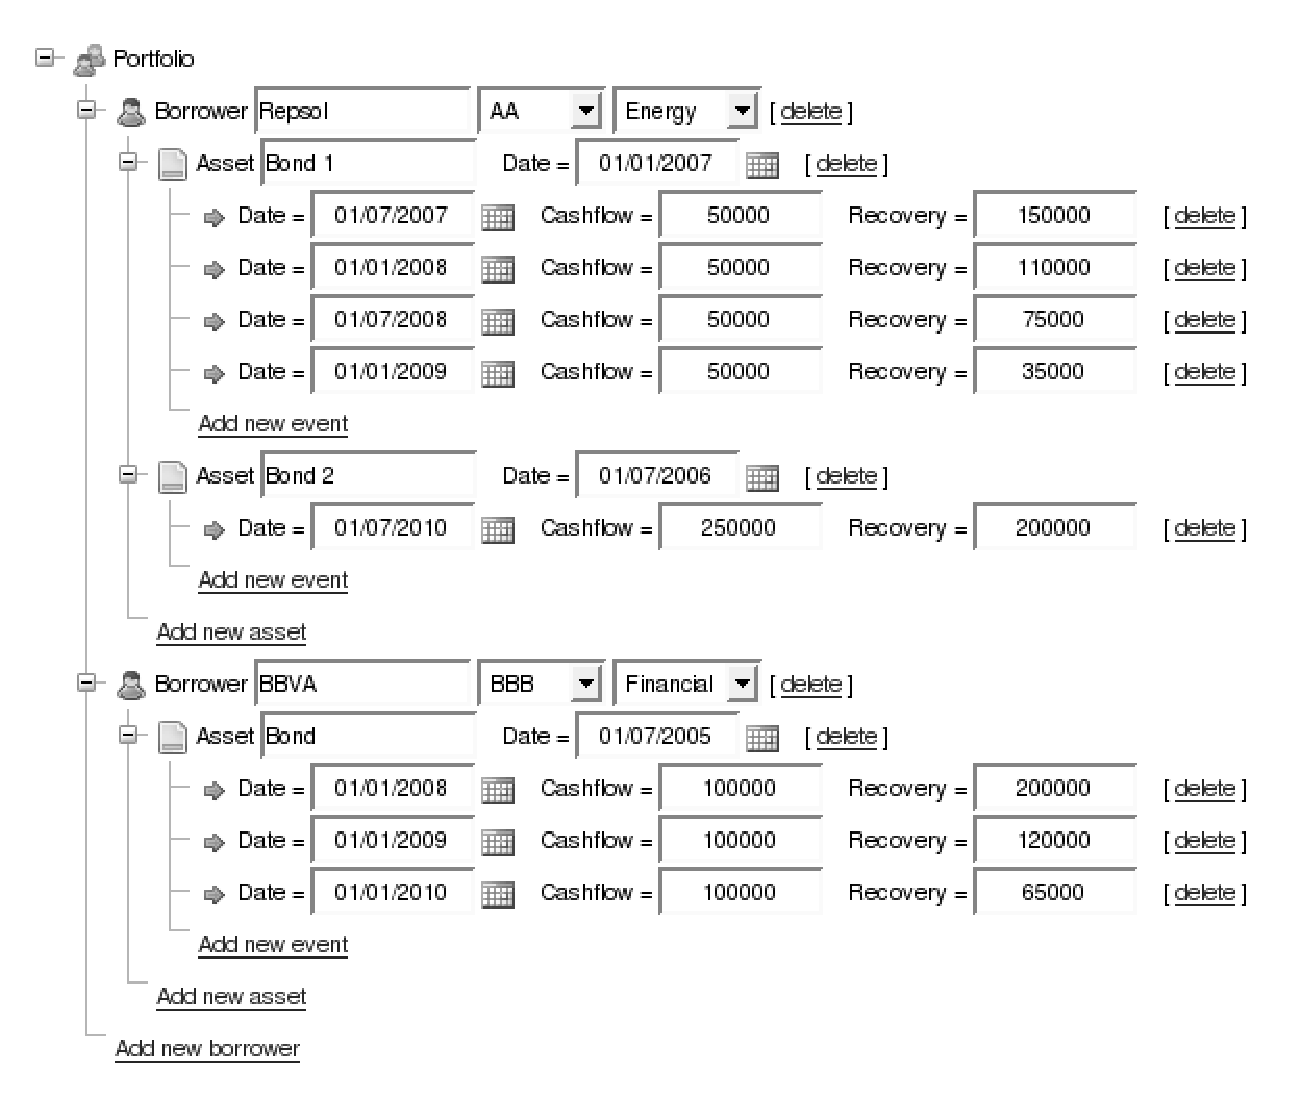
\includegraphics[height=11cm, angle=0]{./images/portfolio.eps}
\caption{Portfolio example}
\label{portfolio}
\end{center}
\end{figure}

Cashflow indicates the cash given to the borrower (negative amounts) and the
cash received from borrower (positive amounts) at each date (see figure\ref{cashflow}).
\newline

\begin{figure}[!hb]
\begin{center}
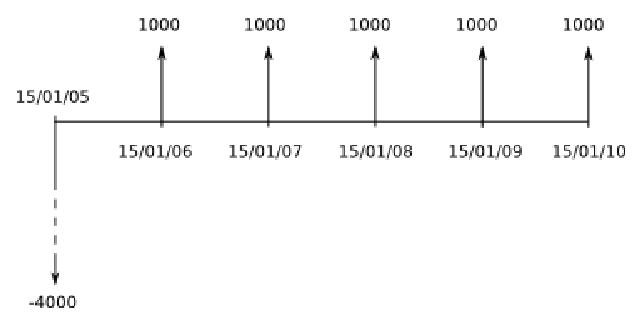
\includegraphics[width=7cm, angle=0]{./images/cashflow.eps}
\caption{Asset cashflow example}
\label{cashflow}
\end{center}
\end{figure}

Recovery indicates the cash recovered (after to take legal action against the 
borrower) if the borrower default at this date (see figure\ref{recovery}).
\newline

\begin{figure}[!hb]
\begin{center}
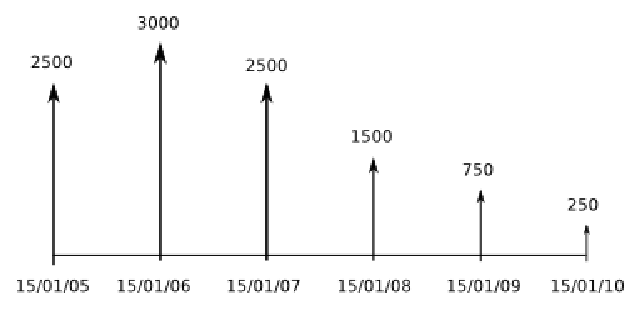
\includegraphics[width=7cm, angle=0]{./images/recovery.eps}
\caption{Asset recovery example}
\label{recovery}
\end{center}
\end{figure}

If a borrower defaults, the loss due to this default is the sum of all remaining
cashflows at default time minus the recovery at default time.


%===========================================================================
\section{Resolution}

\begin{figure}[!hb]
\begin{center}
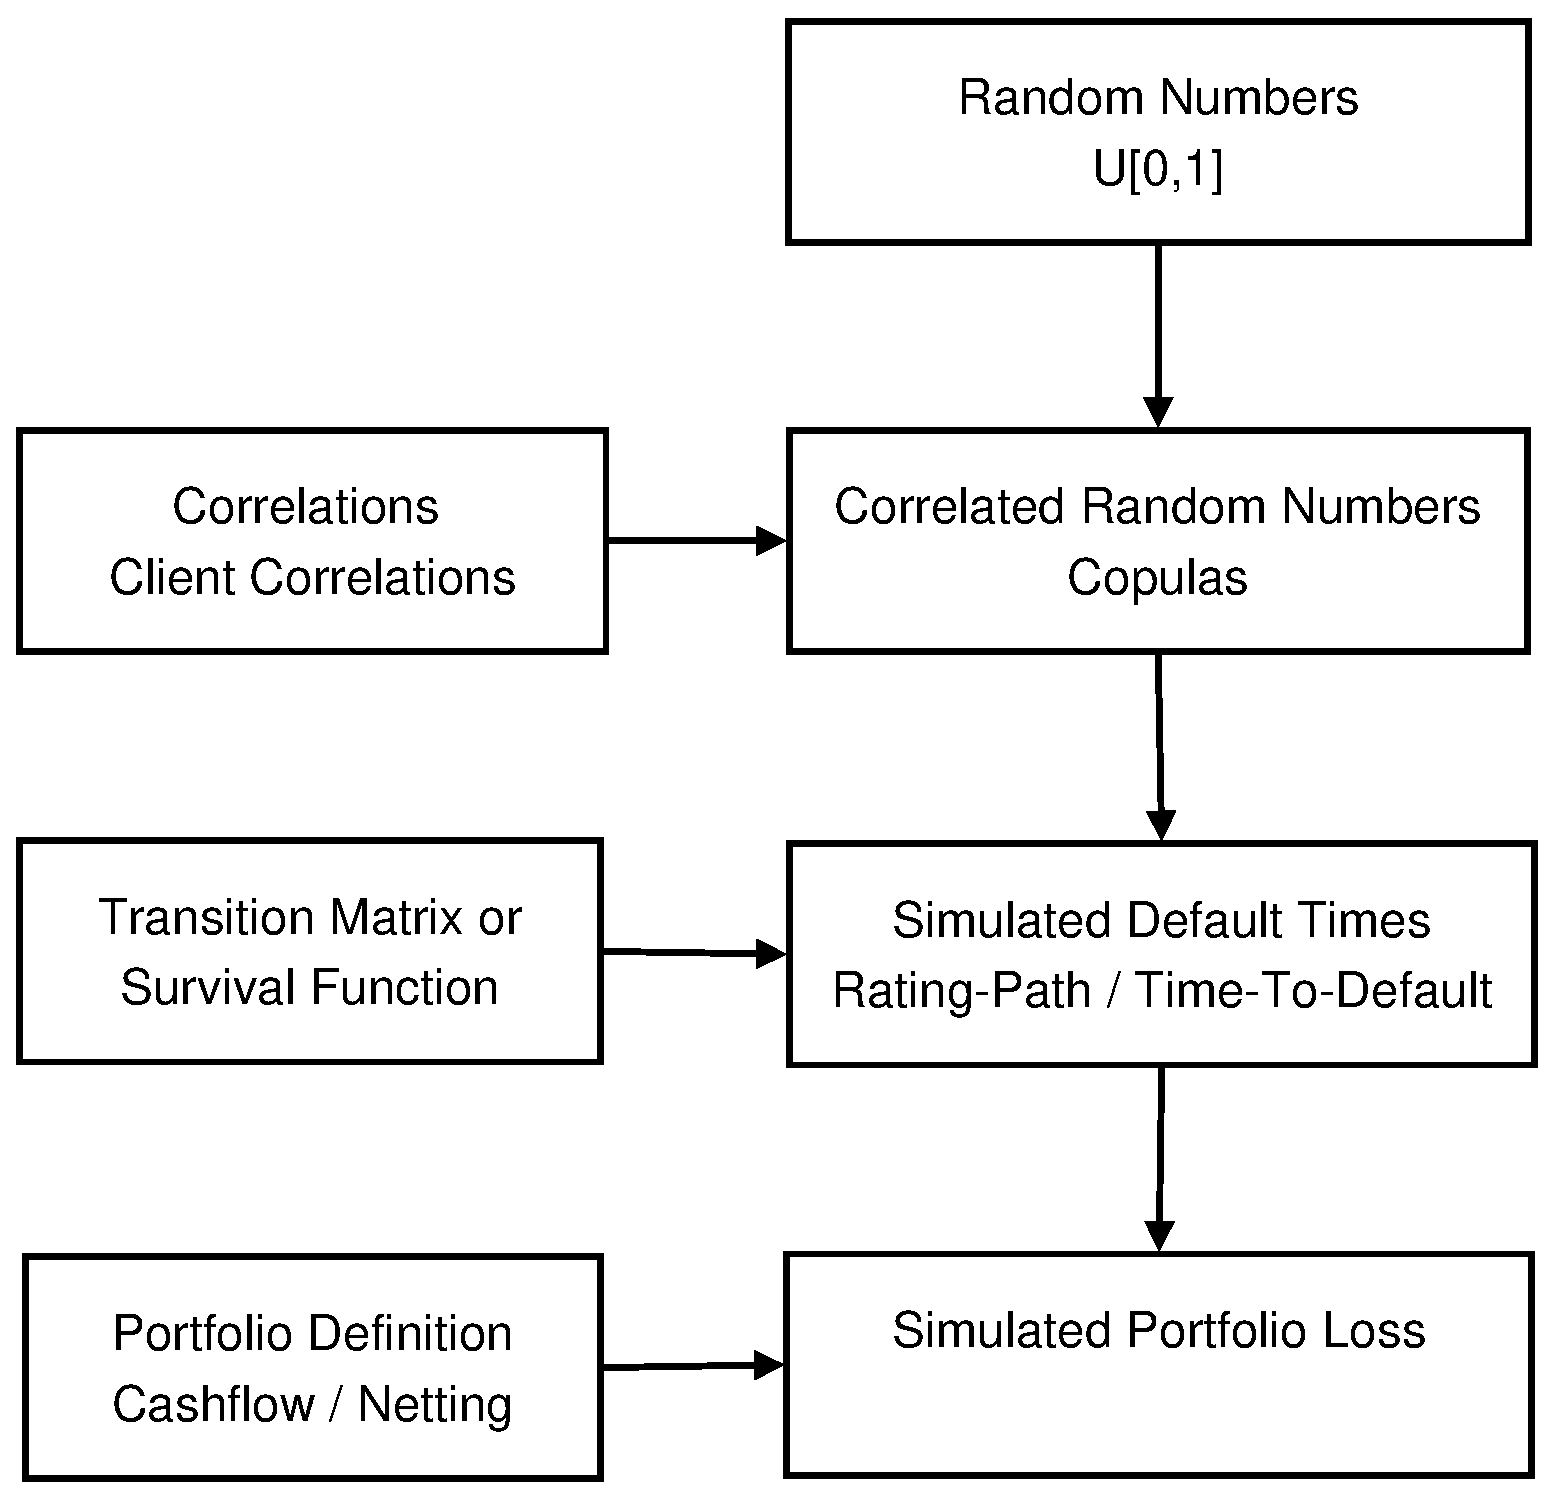
\includegraphics[width=10cm,angle=0]{./images/esquema1.eps}
\caption{Monte Carlo simulation schema}
\label{fig:mcschema1}
\end{center}
\end{figure}

%---------------------------------------------------------------------------
\subsection{Correlation matrix between borrowers}
\label{tcorrel}
We need translate the correlations between sectors to a correlations between
borrowers. Suppose that we have $n$ borrowers and $m$ sectors. Each borrower
belongs to a sector. Correlations between sectors are known:

\begin{center}
\begin{tabular}[]{c|ccc}
             & $Sector_1$     & $\dots$  & $Sector_{m}$   \cr
\hline
$Sector_1$   & $\rho_{1,1}$ & $\dots$  & $\rho_{1,m}$ \cr
$\vdots$     & $\vdots$     & $\ddots$ & $\vdots$     \cr
$Sector_{m}$ & $\rho_{1,m}$ & $\dots$  & $\rho_{m,m}$ \cr
\end{tabular}
\end{center}

where $\rho_{i,j} = Corr(Sector_i, Sector_j)$. We sort the borrowers so that
at the beginning are those of sector $1$ and at the end those of sector $m$. 
Then we create the borrowers correlation matrix taking as correlation between
two borrowers the correlation between his sectors.

\begin{displaymath}
\begin{array}{c}
\left(
\begin{array}{ccccccccccc}
1           & \dots    & \rho_{1,1}  &          & \rho_{1,k}  & \dots   & \rho_{1,k}  &         & \rho_{1,m}  & \dots      & \rho_{1,m}  \cr
\vdots      & \ddots   & \vdots      &          & \vdots      &         & \vdots      &         & \vdots      &            & \vdots      \cr
\rho_{1,1}  & \dots    & 1           &          & \rho_{1,k}  & \dots   & \rho_{1,k}  &         & \rho_{1,m}  & \dots      & \rho_{1,m}  \cr

            &          &             & \ddots   &             &         &             &         &             &            &             \cr

\rho_{1,k}  & \dots    & \rho_{1,k}  &          & 1           & \dots   & \rho_{k,k}  &         & \rho_{k,m}  & \dots      & \rho_{k,m}  \cr
\vdots      & \ddots   & \vdots      &          & \vdots      & \ddots  & \vdots      &         & \vdots      &            & \vdots      \cr
\rho_{1,k}  & \dots    & \rho_{1, }  &          & \rho_{k,k}  & \dots   & 1           &         & \rho_{k,m}  & \dots      & \rho_{k,m}  \cr

            &          &             &          &             &         &             & \ddots  &             &            &             \cr

\rho_{1,m}  & \dots    & \rho_{1,m}  &          & \rho_{k,m}  & \dots   & \rho_{k,m}  &         & 1           & \dots      & \rho_{m,m}  \cr
\vdots      & \ddots   & \vdots      &          & \vdots      & \ddots  & \vdots      &         & \vdots      & \ddots     & \vdots      \cr
\rho_{1,m}  & \dots    & \rho_{1,m}  &          & \rho_{k,m}  & \dots   & \rho_{k,m}  &         & \rho_{m,m}  & \dots      & 1           \end{array}
\right)
\end{array}
\end{displaymath}

Observe that this is a correlation matrix (symmetric, definite positive, 
$|\rho_{i,j}| < 1$, $|\rho_{i,i}| = 1$) composed by blocks. We will use this 
characteristic to adapt the Cholesky algorithm with the aim to improve memory 
size and speed.

%---------------------------------------------------------------------------
\subsection{Mapping losses at time nodes}
Because we want a very fast implementation we precompute losses for each asset 
at fixed time nodes. Time nodes can be distinct than cashflow or recovery dates. 
The following paragraphs tells how compute losses at time nodes.

%...........................................................................
\subsubsection{Recovery at time nodes}
We considerer the recovery at time node $k$ as the closest asset recovery by 
right. If time node $k$ is previous to the first asset event then the recovery 
value at time node $k$ is $0$. If time node $k$ is later to the last asset event 
then the recovery value at time node $k$ is $0$. Figure \ref{recoverymapping} 
shows recovery displayed in figure \ref{recovery} mapped to biannual time nodes.

\begin{figure}[!hb]
\begin{center}
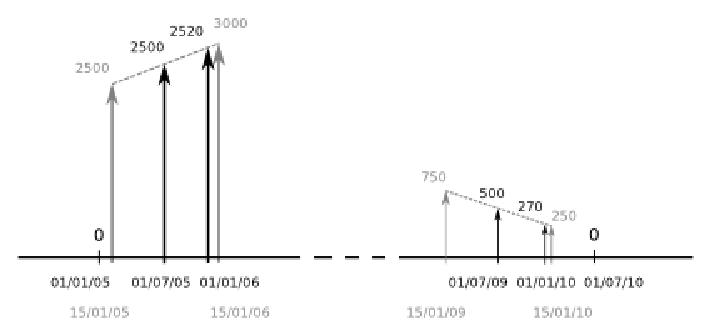
\includegraphics[width=12cm, angle=0]{./images/recoverymapping.eps}
\caption{Asset recoveries mapped to time nodes}
\label{recoverymapping}
\end{center}
\end{figure}

%...........................................................................
\subsubsection{Losses at time nodes}
If borrower defaults before the date of asset risk assumption then loss is $0$.
If borrower defaults after asset finalization date then loss is $0$. 
If borrower defaults at time node $k$ and exists pending cashflows then loss is 
the sum of all pending cashflows minus the recovery at time node $k$.
Figure \ref{lossesmapping} shows asset loss mapped to biannual time nodes of asset
displayed at figures \ref{cashflow}, \ref{recovery} and \ref{recoverymapping}.

\begin{figure}[!hb]
\begin{center}
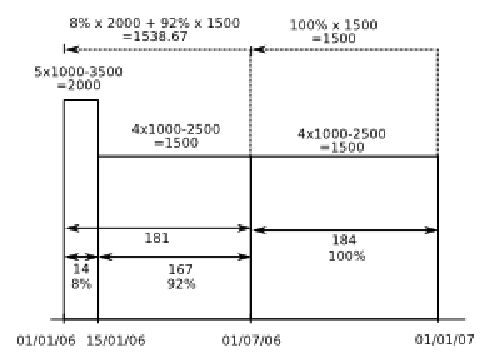
\includegraphics[width=12cm, angle=0]{./images/lossesmapping.eps}
\caption{Asset losses mapped to time nodes}
\label{lossesmapping}
\end{center}
\end{figure}

%---------------------------------------------------------------------------
\subsection{Monte Carlo simulation}
Monte Carlo methods \cite{mc:mervyn} are class of computational algorithms for 
simulating the behavior of various physical and mathematical systems. 
Each simulation consist to compute a random default time for each borrower and
found the portfolio loss value. We need that every default time fulfill the
borrower survival functions and the borrowers correlation matrix. This is 
achieved with the simulation of copulas. A copula \cite{copu:pitfalls} 
\cite{copu:wang}is a multivariate random variable where each component is a 
uniform $U[0,1]$.

%...........................................................................
\subsubsection{Random numbers generation}
Each simulation requires a set of random numbers between $[0, 1]$ correlated by 
the borrowers correlation matrix (see section \ref{tcorrel}), $\Sigma_1$. 
We generate them using the gaussian copula simulation algorithm:

\paragraph{Step 1.} We create the covariance\footnote{Correlation and covariance 
matrix are the same because diagonal elements are $1$.} matrix $\Sigma_2$ mapping 
$\Sigma_1$ component by component:
\begin{displaymath}
\Sigma_2 = \left( 
\begin{array}{cccc}
2 sin(\frac{\pi}{6})           & 2 sin(\rho_{12} \frac{\pi}{6}) & \ldots & 2 sin(\rho_{1n} \frac{\pi}{6})\cr
2 sin(\rho_{12} \frac{\pi}{6}) & 2 sin(\frac{\pi}{6})           & \ldots & 2 sin(\rho_{2n} \frac{\pi}{6})\cr
\vdots                         & \vdots                         & \ddots  & \vdots   \cr
2 sin(\rho_{1n} \frac{\pi}{6}) & 2 sin(\rho_{2n} \frac{\pi}{6}) & \ldots & 2 sin(\frac{\pi}{6})
\end{array}
\right)
\end{displaymath}
Observe that $\Sigma_2$ have diagonal elements with $1$ because $2 sin(\frac{\pi}{6}) = 1$.

\paragraph{Step 2.} We apply Cholesky to $\Sigma_2$, then $\Sigma_2 = B \cdot B^{\top}$, 
where:
\begin{displaymath}
B = 
\left(
\begin{array}{cccc}
b_{11}   & 0        & \ldots & 0       \cr
b_{21}   & b_{22}   & \ldots & 0       \cr
\vdots  & \vdots  & \ddots & \vdots \cr
b_{n1}   & b_{n2}   & \ldots & b_{nn}
\end{array}
\right)
\end{displaymath}

\paragraph{Step 3.} We simulates\footnote{The algorithm used to simulates a $N(0,1)$
is explained in appendix \ref{ap:normsim}} a $N(0,1)$ $n$ times:
\begin{displaymath}
\vec{Y} =
\left(
\begin{array}{c}
y_1 \cr
\vdots \cr
y_n
\end{array}
\right) 
\qquad y_k \sim N(0,1) \textrm{ independents}
\end{displaymath}

\paragraph{Step 4.} We simulate a normal multivariate $\vec{Z} \sim N(\vec{0}, \Sigma_2)$ 
doing:
\begin{displaymath}
B \cdot \vec{Y} 
=
\left(
\begin{array}{cccc}
b_{11}   & 0        & \ldots & 0       \cr
b_{21}   & b_{22}   & \ldots & 0       \cr
\vdots  & \vdots  & \ddots & \vdots \cr
b_{n1}   & b_{n2}   & \ldots & b_{nn}
\end{array}
\right)
\left(
\begin{array}{c}
y_1 \cr
\vdots \cr
y_n
\end{array}
\right) 
=
\left(
\begin{array}{c}
z_1 \cr
\vdots \cr
z_n
\end{array}
\right) 
= 
\vec{Z}
\end{displaymath}

\paragraph{Step 5.} Finally we obtain the copula, $\vec{U}$.
\begin{displaymath}
\left(
\begin{array}{c}
\Phi(z_1) \cr
\vdots \cr
\Phi(z_n)
\end{array}
\right) 
=
\left(
\begin{array}{c}
u_1 \cr
\vdots \cr
u_n
\end{array}
\right) 
=
\vec{X} 
\end{displaymath}
where $\Phi(x)$ is the $N(0,1)$ cumulative distribution function.
\begin{displaymath}
\Phi(x) = \int_{-\infty}^{x} \frac{1}{\sqrt{2 \pi}} e^{-\frac{t^2}{2}} dt
\end{displaymath}

Steps 1 and 2 are done only one time previous to simulation. The rest of steps
are performed for every Monte Carlo simulation.
\newline

In appendix \ref{ap:cholblock} is described a Cholesky decomposition adapted to 
block matrix that allows to work with matrix of size bigger than $50000$.

%...........................................................................
\subsubsection{Default time simulation}
Given the borrower $k$ and a random number $u_k \in [0,1]$ (generated using a 
copula in the previous step) we simulates the default time considering the 
inverse of the borrower survival function at $u_k$. Figure \ref{simttd} shows 
this in a graphic manner.

\begin{figure}[!hb]
\begin{center}
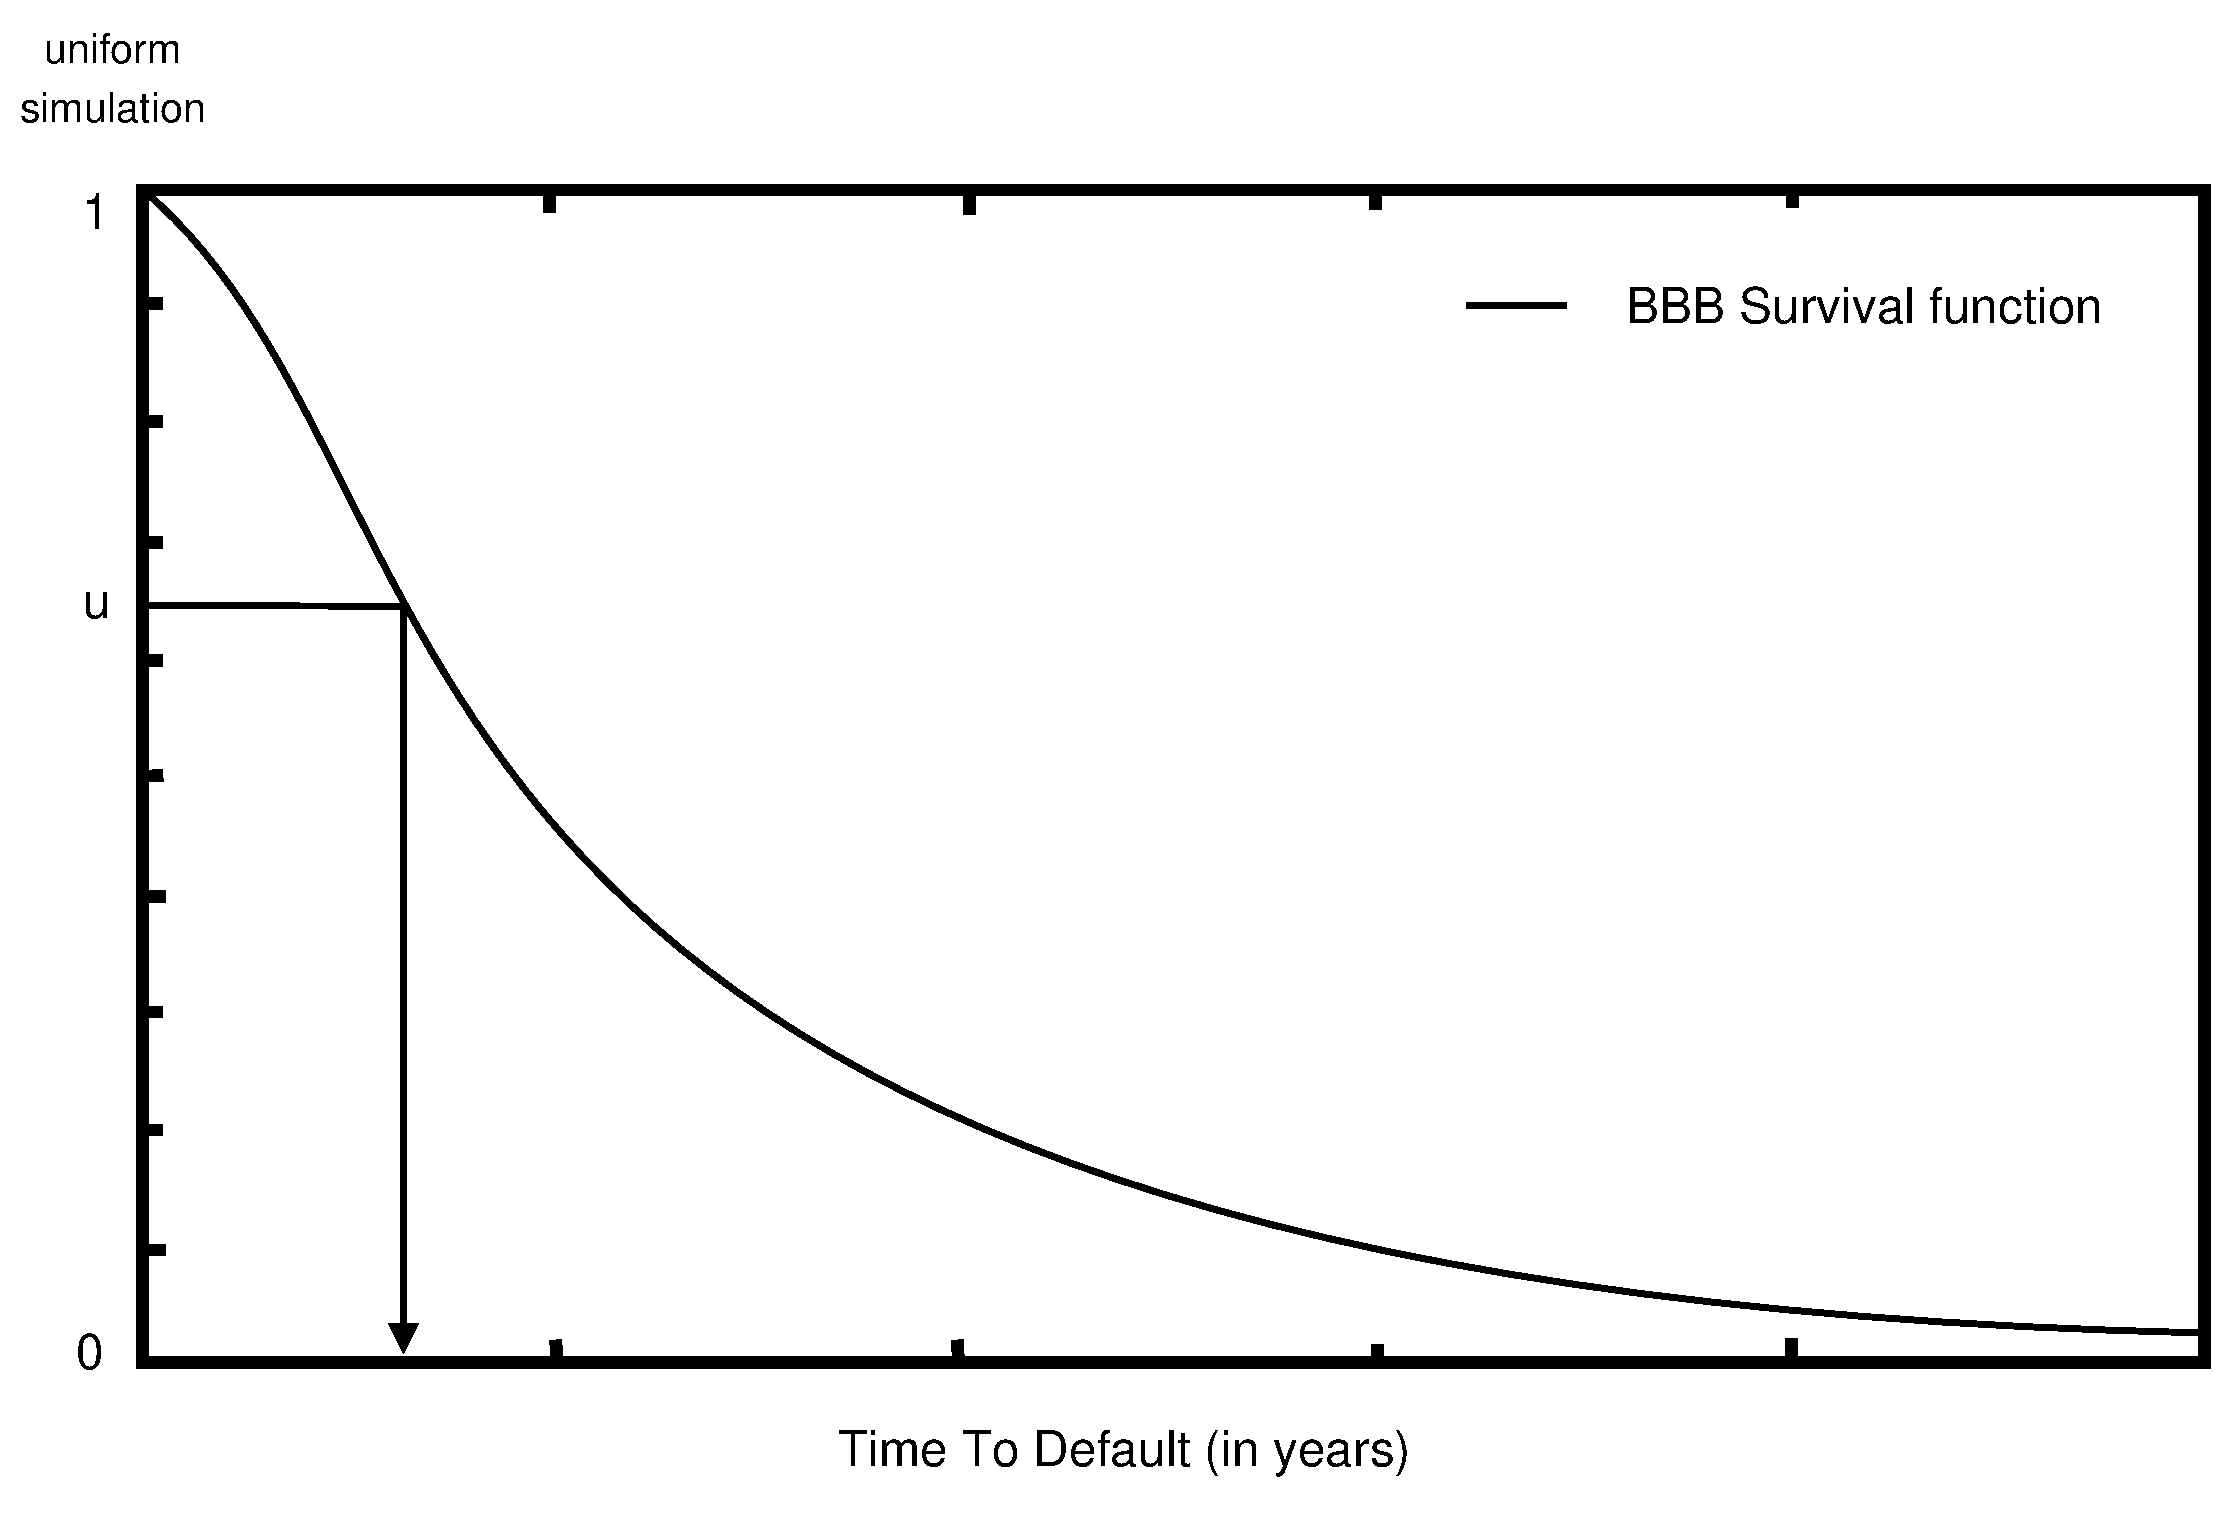
\includegraphics[width=10cm,angle=0]{./images/simttd.eps}
\caption{Default time simulation with initial rating $BBB$}
\label{simttd}
\end{center}
\end{figure}

%...........................................................................
\subsubsection{Portfolio loss evaluation}
At this point, given any borrower, we have a simulated default time. We map
this default time to time node closest by the right where we have the precomputed 
losses for his assets. To obtain the simulated portfolio loss value we sum all 
assets losses and we kept this value in a list.

%---------------------------------------------------------------------------
\subsection{Risk computation}
After $N$ simulations (eg. $20000$, $50000$ or more) we have a list
of numbers, $x_i$, where each number represents a simulated portfolio loss. More 
values imply more accuracy in results. All risk statistics (eg. Expected Loss) 
have an error that will be estimated. First of all we can approximate the 
portfolio loss probability distribution creating an histogram with the simulated 
values. 
\newline

CCruncher uses \emph{R package}\footnote{http://www.r-project.org} to perform 
the statistical computations described in this section.

\begin{figure}[!hb]
\begin{center}
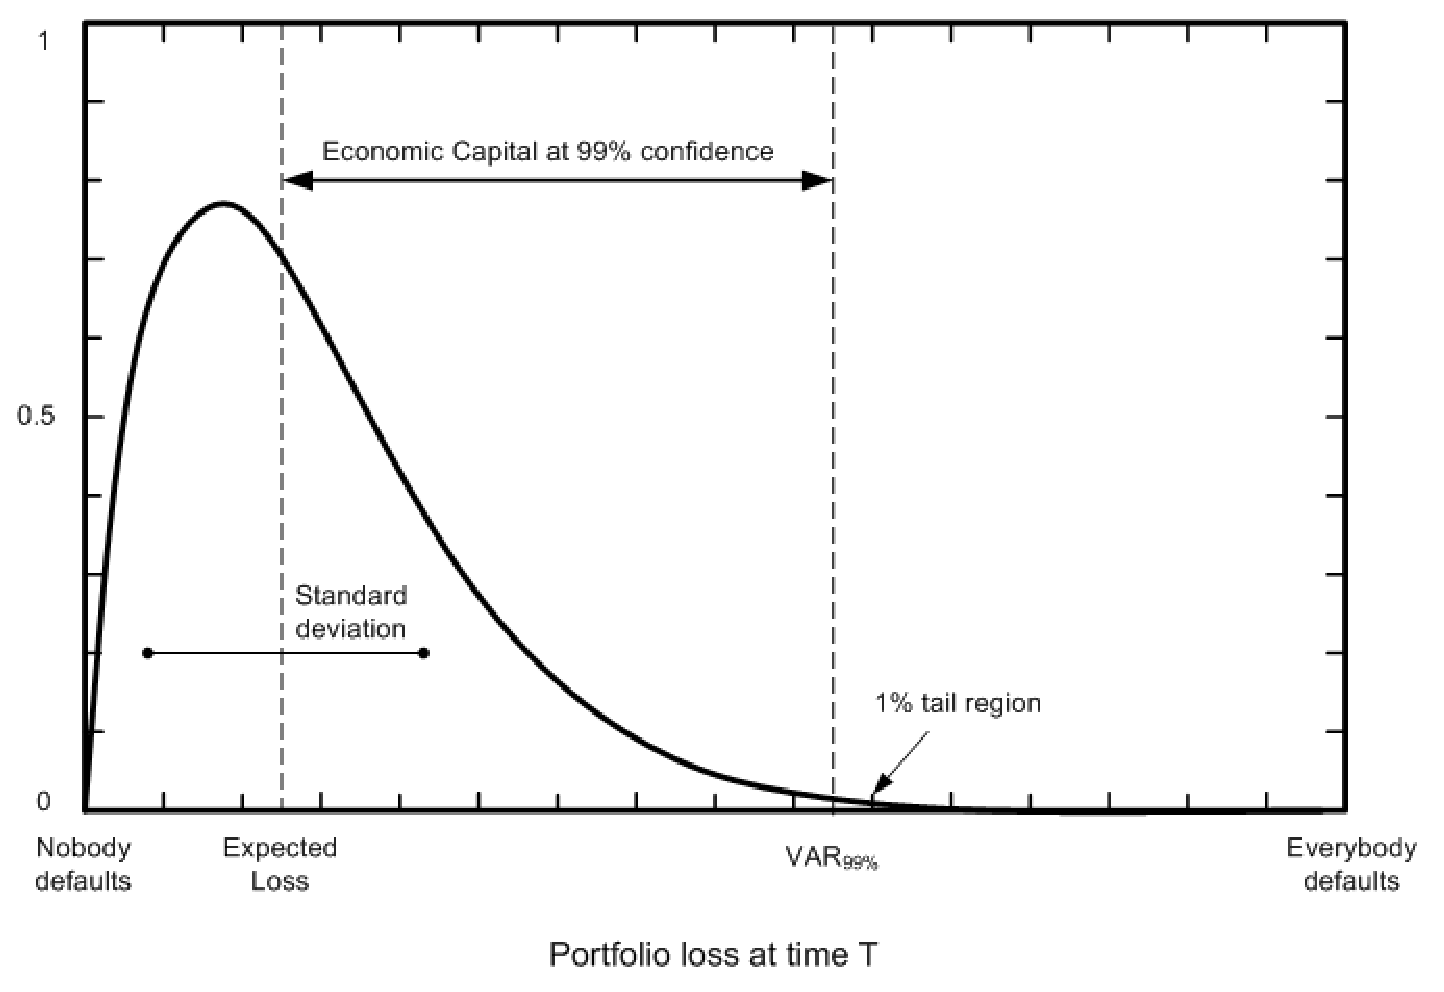
\includegraphics[height=7cm, angle=0]{./images/creditvar.eps}
\caption{Portfolio loss at time $T$}
\label{creditvar}
\end{center}
\end{figure}

%...........................................................................
\subsubsection{Expected Loss}
Expected Loss is the mean of the portfolio loss probability distribution.
Central Limit Theorem \cite{stats:schaum} grants that:

\begin{displaymath}
\mu = \widehat{\mu} \pm \phi^{-1}\left(\frac{1-\alpha}{2}\right) \cdot \frac{\widehat{\sigma}}{\sqrt{N}}
\end{displaymath}
where $\alpha$ is the confidence level for error, $\phi^{-1}$ the N(0,1) inverse 
cumulative distribution function and $\widehat{\mu}$ and $\widehat{\sigma}$ are 
the mean and stddev estimators:

\begin{displaymath}
\widehat{\mu} = \frac{1}{N} \sum_{i=1}^{N} x_i
\end{displaymath}

\begin{displaymath}
\widehat{\sigma} =
\sqrt{\frac{1}{N-1} \sum_{i=1}^{N} \left( x_i - \widehat{\mu} \right)^2} =
\sqrt{\frac{1}{N-1} \left( \sum_{i=1}^{N} x_i^2 - \frac{\left(\sum_{i=1}^{N} x_i \right)^2}{N} \right)}
\end{displaymath}

%...........................................................................
\subsubsection{Portfolio Loss Standard Deviation}
Other usual risk statistic is the portfolio loss standard deviation as measure
of dispersion from mean. Central Limit Theorem \cite{stats:schaum} grants that:

\begin{displaymath}
\sigma = \widehat{\sigma} \pm \phi^{-1}\left(\frac{1-\alpha}{2}\right) \cdot \frac{\widehat{\sigma}}{\sqrt{2N}}
\end{displaymath}

where $\alpha$ is the confidence level for error, $\phi^{-1}$ the N(0,1) inverse 
cumulative distribution function and $\widehat{\sigma}$ is stddev estimator:

\begin{displaymath}
\widehat{\sigma} =
\sqrt{\frac{1}{N-1} \sum_{i=1}^{N} \left( x_i - \widehat{\mu} \right)^2} =
\sqrt{\frac{1}{N-1} \left( \sum_{i=1}^{N} x_i^2 - \frac{\left(\sum_{i=1}^{N} x_i \right)^2}{N} \right)}
\end{displaymath}

%...........................................................................
\subsubsection{Value At Risk}
Value at Risk \cite{var:jorion} is the most used risk value. We note as 
$VAR_{\beta}$ where $\beta$ is the VAR confidence level (eg. VAR at $95\%$).
VAR is another form to say quantile. Then
$VAR_{\beta} = q_{\beta} = \textrm{inf}\{x | F(x) \geq \beta \}$. 

\begin{displaymath}
VAR_{\beta} = \widehat{q_{\beta}} \pm \phi^{-1}\left(\frac{1-\alpha}{2}\right) \cdot \textrm{stderr}(q_{\beta})
\end{displaymath}

where $\alpha$ is the confidence level for error, $\beta$ is the VAR confidence 
level, $\phi^{-1}$ the N(0,1) inverse cumulative distribution function, 
$\widehat{q_{\beta}}$ is the quantile estimator, and $\textrm{stderr}(q_{\beta})$
is a estimation of the standard error.

\begin{displaymath}
\widehat{q_{\beta}} = x_{k:N}
\end{displaymath}
where,
\begin{itemize}
\item $k$ fulfills $\frac{k}{N} \leq \beta < \frac{k+1}{N}$
\item $x_{k:N}$ is the $k$-th element of ascendent sorted values
\end{itemize}

We determine $\textrm{stderr}(q_{\beta})$ using Maritz-Jarret method described
in \cite{quant:algor}.

\begin{eqnarray}
M   & = & [N \beta + 0.5] \nonumber \\
a   & = & M - 1 \nonumber \\
b   & = & N - M \nonumber \\
W_i & = & B(a,b,\frac{i+1}{N}) - B(a,b,\frac{i}{N}) \nonumber \\
C_k & = & \sum_{i=1}^{N} W_i \cdot x_i \nonumber
\end{eqnarray}

where $[x]$ is the integer part of $x$ and $B(a,b,x)$ is the incomplete beta 
function:

\begin{displaymath}
B(a,b,x)=\frac{\Gamma(a+b)}{\Gamma(a)\Gamma(b)}\int_0^x t^{a-1} (1-t)^{b-1} dt
\end{displaymath}

Then,
\begin{displaymath}
\textrm{stderr}(q_{\beta}) = \sqrt{C_2 - C_1^2}
\end{displaymath}

%...........................................................................
\subsubsection{Expected Shortfall}
VAR is not a distance because it don't fulfills sub-additive property \cite{var:varbad}, 
that is $VAR(A+B) \nleq VAR(A)+VAR(B)$. Expected Shortfall is a consistent risk 
measure \cite{var:eshortfall} similar to VAR. Can be described as the average of 
the $\beta\%$ worst losses.

\begin{displaymath}
ES_{\beta} = \widehat{ES_{\beta}} \pm \phi^{-1}\left(\frac{1-\alpha}{2}\right) \cdot \textrm{stderr}(ES_{\beta})
\end{displaymath}

where $\alpha$ is the confidence level for error, $\beta$ is the ES confidence 
level, $\phi^{-1}$ the N(0,1) inverse cumulative distribution function, 
$\widehat{ES_{\beta}}$ is the ES estimator and $\textrm{stderr}(ES_{\beta})$
is a estimation of the standard error.
\newline

We select the simulation portfolio loss values that are bigger than $VAR_{\beta}$.
\begin{displaymath}
y_1, y_2, y_3, \cdots, y_K \qquad \textrm{where} \quad y_i > VAR_{\beta}
\end{displaymath}

Then,

\begin{displaymath}
\widehat{ES_{\beta}} = \frac{1}{K} \sum_{i=1}^{K} y_i
\end{displaymath}

\begin{displaymath}
\textrm{stderr}(ES_{\beta}) =
\frac{\sqrt{\frac{1}{K-1} \sum_{i=1}^{K} \left( y_i - \widehat{ES_{\beta}} \right)^2}}{\sqrt{K}} =
\frac{\sqrt{\frac{1}{K-1} \left( \sum_{i=1}^{K} y_i^2 - \frac{\left(\sum_{i=1}^{K} y_i \right)^2}{K} \right)}}{\sqrt{K}}
\end{displaymath}

%...........................................................................
\subsubsection{Economic Capital}
We can compute the Economic Capital at confidence level $\beta$ as:

\begin{displaymath}
\textrm{Economic Capital} = VAR_{\beta} - \textrm{Expected Loss}
\end{displaymath}

%...........................................................................

\begin{figure}[p]
\begin{center}
\includegraphics[width=12cm,angle=0]{./images/report.eps}
\caption{CCruncher results}
\label{report}
\end{center}
\end{figure}


%===========================================================================
\section{Other considerations}
CCruncher takes other considerations that they have not been exposed
until this moment with the purpose of simplifying the content.

%---------------------------------------------------------------------------
\subsection{Risk aggregation}
CCruncher simulates the whole portfolio loss at time $T$. Also allows simulates 
(in the same execution), subportfolios defining one or more aggregators. 
Consequently you can determine what are the branches (or products or borrowers 
or regions or assets, etc.) that contributes to increase the risk of your portfolio.
Every subportfolio have its own list of simulated values that can be processed
to obtain the risk indicators for this subportfolio.

%---------------------------------------------------------------------------
\subsection{Time updates}
CCruncher can considerer that money value decrease along the time following a fixed 
curve (eg. yield curve). CCruncher allows to specify the yield curve and perform
all computations that involves cash transport along the time (recovery mapping, 
losses mapping and portfolio value at time $T$) taking into account this fact.
The time transport coeficient is determined using the compound interest formula:

\begin{displaymath}
\Upsilon(r, t_0,t_1) = (1+r)^{(t_1-t_0)}
\end{displaymath}

%---------------------------------------------------------------------------
\subsection{Antithetic technique}
The random number generation using a copula is time expensive. Gaussian copula
is symmetric, that means that $(u_1, u_2, \cdots, u_N)$ is equiprobable to
$(1-u_1, 1-u_2, \cdots, 1-u_N)$. In CCruncher antithetic mode, each copula 
generation is used $2$ times, as $(u_1, u_2, \cdots, u_N)$ and 
as $(1-u_1, 1-u_2, \cdots, 1-u_N)$ reducing in this way the number of generated
copulas.

%---------------------------------------------------------------------------
\subsection{Parallel computing}
Monte Carlo problems are embarrassingly parallel problems.
In the jargon of parallel computing, an embarrassingly parallel workload 
(or embarrassingly parallel problem) is one for which no particular effort 
is needed to segment the problem into a very large number of parallel tasks, 
and there is no essential dependency (or communication) between those parallel 
tasks.
\newline

In CCruncher a master sends the RNG seed to each slave 
($seed_i = seed + i \cdot 30001$) and wait results (portfolio loss simulated
values) from slaves that put in a file. When stop criteria is achieved 
(execution time exceded or number of required simulations achieved) send a 
stop signal to slaves and leaves.

%===========================================================================
\newpage
\appendix
\section{Appendices}

%---------------------------------------------------------------------------
\subsection{How simulate a N(0,1)}
\label{ap:normsim}

In order to simulate $Z \sim N(\mu, \sigma^2)$ values we use:

\begin{displaymath}
z = \mu + \sigma\cdot \sqrt{-2 ln(u_1)} \cdot cos(2 \pi \cdot u_2)
\qquad u_1, u_2 \sim U[0,1]
\end{displaymath}

Where $u_i$ are generated by a Mersenne Twister random number generator.

%---------------------------------------------------------------------------
\subsection{Cholesky decomposition for block matrix}
\label{ap:cholblock}

Cholesky algorithm decompose a symmetric positive definite matrix into a lower
triangular matrix and the transpose of the lower triangular matrix. Algorithm 
description can be found in \emph{Numerical Recipes in C}\footnote{http://www.nr.com}.

\begin{displaymath}
U^{\top} \cdot U = A
\end{displaymath}

If we have a portfolio of $50000$ borrowers, our correlation matrix size will
be a $50000 \times 50000$ matrix. This requires up to 19 Gb. of RAM memory and
multiply this matrix by a vector suppose $2500000000$ multiplications.
\newline

We adapt the Cholesky algorithm in order to consider that borrower correlations
matrix is a block matrix with $1$'s in diagonal like this example:

\begin{displaymath}
A = \left(
\begin{array}{cccc|ccc}
1   & 0.5 & 0.5 & 0.5 & 0.1 & 0.1 & 0.1 \cr
0.5 & 1   & 0.5 & 0.5 & 0.1 & 0.1 & 0.1 \cr
0.5 & 0.5 & 1   & 0.5 & 0.1 & 0.1 & 0.1 \cr
0.5 & 0.5 & 0.5 & 1   & 0.1 & 0.1 & 0.1 \cr
\hline
0.1 & 0.1 & 0.1 & 0.1 & 1   & 0.3 & 0.3 \cr
0.1 & 0.1 & 0.1 & 0.1 & 0.3 & 1   & 0.3 \cr
0.1 & 0.1 & 0.1 & 0.1 & 0.3 & 0.3 & 1
\end{array}
\right)
\end{displaymath}

We decompose the previous matrix using the standard Cholesky decomposition:

\begin{displaymath}
U = \left(
\begin{array}{cccc|ccc}
 1.00000 & 0.50000 & 0.50000 & 0.50000 & 0.10000 & 0.10000 & 0.10000 \cr
 0       & 0.86603 & 0.28868 & 0.28868 & 0.05774 & 0.05774 & 0.05774 \cr
 0       & 0       & 0.81650 & 0.20412 & 0.04082 & 0.04082 & 0.04082 \cr
 0       & 0       & 0       & 0.79057 & 0.03162 & 0.03162 & 0.03162 \cr
\hline
 0       & 0       & 0       & 0       & 0.99197 & 0.28630 & 0.28630 \cr
 0       & 0       & 0       & 0       & 0       & 0.94975 & 0.21272 \cr
 0       & 0       & 0       & 0       & 0       & 0       & 0.92563
\end{array}
\right)
\end{displaymath}

Observe that $U$ have repeated elements that allows to kept in RAM memory like this:

\begin{displaymath}
U = \left|
\begin{array}{c|cc}
 1.00000 & 0.50000 & 0.10000 \cr
 0.86603 & 0.28868 & 0.05774 \cr
 0.81650 & 0.20412 & 0.04082 \cr
 0.79057 & 0       & 0.03162 \cr
 0.99197 & 0       & 0.28630 \cr
 0.94975 & 0       & 0.21272 \cr
 0.92563 & 0       & 0
\end{array}
\right|
\end{displaymath}

that is, for each row we kept the diagonal value and the value of each sector. 
With this strategy the required memory size is $N \times (M+1)$ where $N$ is
the number of borrowers and $M$ the number of sectors. With this consideration
the memory required to store a $50000$ borrowers correlation matrix is only
$4.2$ Mb.
\newline

We use the fact that matrix $U$ have repeated elements to reduce the number of 
operations required to multiply $A$ by a vector. Let us to see an example:

\begin{displaymath}
\begin{array}{l}
(U \cdot x)_2 =  0.86603 \cdot x_2 + 0.28868 \cdot x_3 + 0.28868 \cdot x_4 + \cr
                 0.05774 \cdot x_5 + 0.05774 \cdot x_6 + 0.05774 \cdot x_7 \cr
              = 0.86603 \cdot x_2 + 2\cdot 0.28868 \cdot (x_3 + x_4) + 3 \cdot 0.05774 \cdot (x_5 + x_6 + x_7)
\end{array}
\end{displaymath}

With this consideration we can reduce the number of operations from $N^2$ to 
$N \times (M+1)$ where $N$ is the number of borrowers and $M$ the number of 
sectors. In the $50000$ borrowers example, the operations number reduce from 
$2500000000$ to only $500000$.

%---------------------------------------------------------------------------
\subsection{From transition matrix to survival function}
\label{ap:tmatrix}
The $T$-years transition matrix gives the probability to jump from rating $r_i$ 
to rating $r_j$ in a term of $T$ years.

\begin{displaymath}
M_T = \left(
\begin{array}{ccc}
m_{1,1} & \dots  & m_{1,n} \cr
\vdots & \ddots & \vdots \cr
m_{n,1} & \dots  & m_{n,n} 
\end{array}
\right)
\qquad
m_{i,j} = P(r_i \to r_j;T)
\end{displaymath}

where $n$ is the number of ratings and $m_{i,j}$ is the probability that a
borrower with rating $r_i$ jumps to $r_j$ in $T$ years.
Figure \ref{tmatrix1} shows a transition matrix example with the probability 
that a borrower with rating $AA$ jumps to rating $B$ in $1$ year is $0.14\%$.
\newline

\begin{figure}[!hb]
\begin{center}
\begin{tabular}[]{l|rrrrrrrr}
        &      AAA &       AA &        A &      BBB &       BB &        B &      CCC &  Default \cr
\hline
AAA     &  $90.81$ &   $8.33$ &   $0.68$ &   $0.06$ &   $0.12$ &   $0.00$ &   $0.00$ &   $0.00$ \cr
 AA     &   $0.70$ &  $90.65$ &   $7.79$ &   $0.64$ &   $0.06$ &   $0.14$ &   $0.02$ &   $0.00$ \cr
  A     &   $0.09$ &   $2.27$ &  $91.05$ &   $5.52$ &   $0.74$ &   $0.26$ &   $0.01$ &   $0.06$ \cr
BBB     &   $0.02$ &   $0.33$ &   $5.95$ &  $86.93$ &   $5.30$ &   $1.17$ &   $0.12$ &   $0.18$ \cr
 BB     &   $0.03$ &   $0.14$ &   $0.67$ &   $7.73$ &  $80.53$ &   $8.84$ &   $1.00$ &   $1.06$ \cr
  B     &   $0.00$ &   $0.11$ &   $0.24$ &   $0.43$ &   $6.48$ &  $83.46$ &   $4.07$ &   $5.21$ \cr
CCC     &   $0.22$ &   $0.00$ &   $0.22$ &   $1.30$ &   $2.38$ &  $11.24$ &  $64.86$ &  $19.78$ \cr
Default &   $0.00$ &   $0.00$ &   $0.00$ &   $0.00$ &   $0.00$ &   $0.00$ &   $0.00$ & $100.00$
\end{tabular}
\caption{$1$-year transition matrix}
\label{tmatrix1}
\end{center}
\end{figure}

Transition matrix can be scaled in time using the following rules:

\begin{equation}
\label{sttm}
\begin{array}{l}
M_{T_1+T_2} = M_{T_1} \cdot M_{T_2} \nonumber \\
M_{k \cdot T} = M_{T}^k \nonumber \\
M_{\frac{T}{k}} = \sqrt[k]{M_{T}} \nonumber
\end{array}
\end{equation}

The root of matrix can be computed as:

\begin{displaymath}
M = P^{-1} \cdot D \cdot P 
\longrightarrow
M^{\gamma} = P^{-1} \cdot D^{\gamma} \cdot P
\end{displaymath}

where $P$ is a matrix composed by the eigenvectors of $M$ and $D$ is a diagonal 
matrix composed by the eigenvalues of $M$. The inverse of a matrix can be 
computed using the $LU$ decomposition as it explained in \emph{Numerical 
Recipes in C}\footnote{http://www.nr.com}:

\begin{displaymath}
Id = P^{-1} \cdot P = L \cdot U \cdot P
\end{displaymath}

This allows us to compute probability default for any time and any initial rating
(that is, the survival functions) doing:

\begin{displaymath}
Survival(r_i, t) = \left( M_t \right)_{i, n}
\end{displaymath}

where $r_i$ is the initial rating, $t$ is the time, $M_t$ is the transition 
matrix for time $t$ (scaled from $M_T$ using (\ref{sttm})) and $n$ is the 
index of default rating, $r_n$.

%===========================================================================
\newpage
\bibliography{refs}
\bibliographystyle{plain}


\end{document}

